\documentclass[11pt]{scrartcl}
\usepackage[T1]{fontenc}
\usepackage[a4paper, left=3cm, right=2cm, top=2cm, bottom=2cm]{geometry}
\usepackage[activate]{pdfcprot}
\usepackage[ngerman]{babel}
\usepackage[parfill]{parskip}
\usepackage[utf8]{inputenc}
\usepackage{kurier}
\usepackage{amsmath}
\usepackage{amssymb}
\usepackage{xcolor}
\usepackage{epstopdf}
\usepackage{txfonts}
\usepackage{fancyhdr}
\usepackage{graphicx}
\usepackage{prettyref}
\usepackage{hyperref}
\usepackage{eurosym}
\usepackage{setspace}
\usepackage{units}
\usepackage{eso-pic,graphicx}
\usepackage{icomma}
\usepackage{pdfpages}

\definecolor{darkblue}{rgb}{0,0,.5}
\hypersetup{pdftex=true, colorlinks=true, breaklinks=false, linkcolor=black, menucolor=black, pagecolor=black, urlcolor=darkblue}



\setlength{\columnsep}{2cm}


\newcommand{\arcsinh}{\mathrm{arcsinh}}
\newcommand{\asinh}{\mathrm{arcsinh}}
\newcommand{\ergebnis}{\textcolor{red}{\mathrm{Ergebnis}}}
\newcommand{\fehlt}{\textcolor{red}{Hier fehlen noch Inhalte.}}
\newcommand{\betanotice}{\textcolor{red}{Diese Aufgaben sind noch nicht in der Übung kontrolliert worden. Es sind lediglich meine Überlegungen und Lösungsansätze zu den Aufgaben. Es können Fehler enthalten sein!!! Das Dokument wird fortwährend aktualisiert und erst wenn das \textcolor{black}{beta} aus dem Dateinamen verschwindet ist es endgültig.}}
\newcommand{\half}{\frac{1}{2}}
\renewcommand{\d}{\, \mathrm d}
\newcommand{\punkte}{\textcolor{white}{xxxxx}}
\newcommand{\p}{\, \partial}
\newcommand{\dd}[1]{\item[#1] \hfill \\}

\renewcommand{\familydefault}{\sfdefault}
\renewcommand\thesection{}
\renewcommand\thesubsection{}
\renewcommand\thesubsubsection{}


\newcommand{\themodul}{Optische Technologie}
\newcommand{\thetutor}{Prof. Rateike}
\newcommand{\theuebung}{Übung 2}

\pagestyle{fancy}
\fancyhead[L]{\footnotesize{C. Hansen}}
\chead{\thepage}
\rhead{}
\lfoot{}
\cfoot{}
\rfoot{}

\title{\themodul{}, \theuebung{}, \thetutor}


\author{Christoph Hansen \\ {\small \href{mailto:chris@university-material.de}{chris@university-material.de}} }

\date{}


\begin{document}

\maketitle

Dieser Text ist unter dieser \href{http://creativecommons.org/licenses/by-nc-sa/4.0/}{Creative Commons} Lizenz veröffentlicht.

\textcolor{red}{Ich erhebe keinen Anspruch auf Vollständigkeit oder Richtigkeit. Falls ihr Fehler findet oder etwas fehlt, dann meldet euch bitte über den Emailkontakt.}

\tableofcontents


\newpage



\section{Aufgabe 1}


Wir betrachten eine Glasscheibe die mit einer Antireflexschicht aus $MgF_2$ bedampft ist. Die Schicht hat einen Brechungsindex von $n_{AR} = 1,38$ und wirkt gegen die Wellenlänge $\lambda = \unit[550]{nm}$. Zunächst bestimmen wir die Dicke der Antireflexschicht:

\begin{align*}
d &= \frac{\lambda_0}{4 \cdot n_{AR}} = \frac{550 \cdot 10^{-9}}{4 \cdot 1,38} = \unit[99,6]{nm}
\intertext{Diese Schicht erzeugt einen Ganunterschied von $\frac{\lambda}{2} = \unit[275]{nm}$. Der Phasenunterschied ist dann:}
\phi &= \frac{2 \pi}{\lambda} \cdot 275 = \frac{\pi \cdot 550}{\lambda}
\intertext{Mit dem Wissen, das $I \sim \cos^2 \left( \frac{\phi}{2} \right)$ ist, können wir den Verlauf der Intensität abhängig von der Phasenverschiebung darstellen. Beispielhaft habe ich eine Tabelle gebaut:}
\end{align*}

\begin{center}
	\begin{tabular}{|c|c|c|}
		 $\lambda$ & $\phi$ & $I$ \\ 
		 \hline
		400  &  &  \\ 
		$\vdots$  &  &  \\ 
	    700	 &  &  \\ 		
	\end{tabular} 
\end{center}

Wenn man das plottet, dann erhält man einen Graphen , der bei $\unit[550]{nm}$ ein Minimum haben sollte.

Nun schauen wir uns noch an wie gut die Antireflexionsschicht das reflektierte Licht reduziert.


\begin{figure}[h]
	\begin{minipage}[hbt]{5cm}
		\centering
		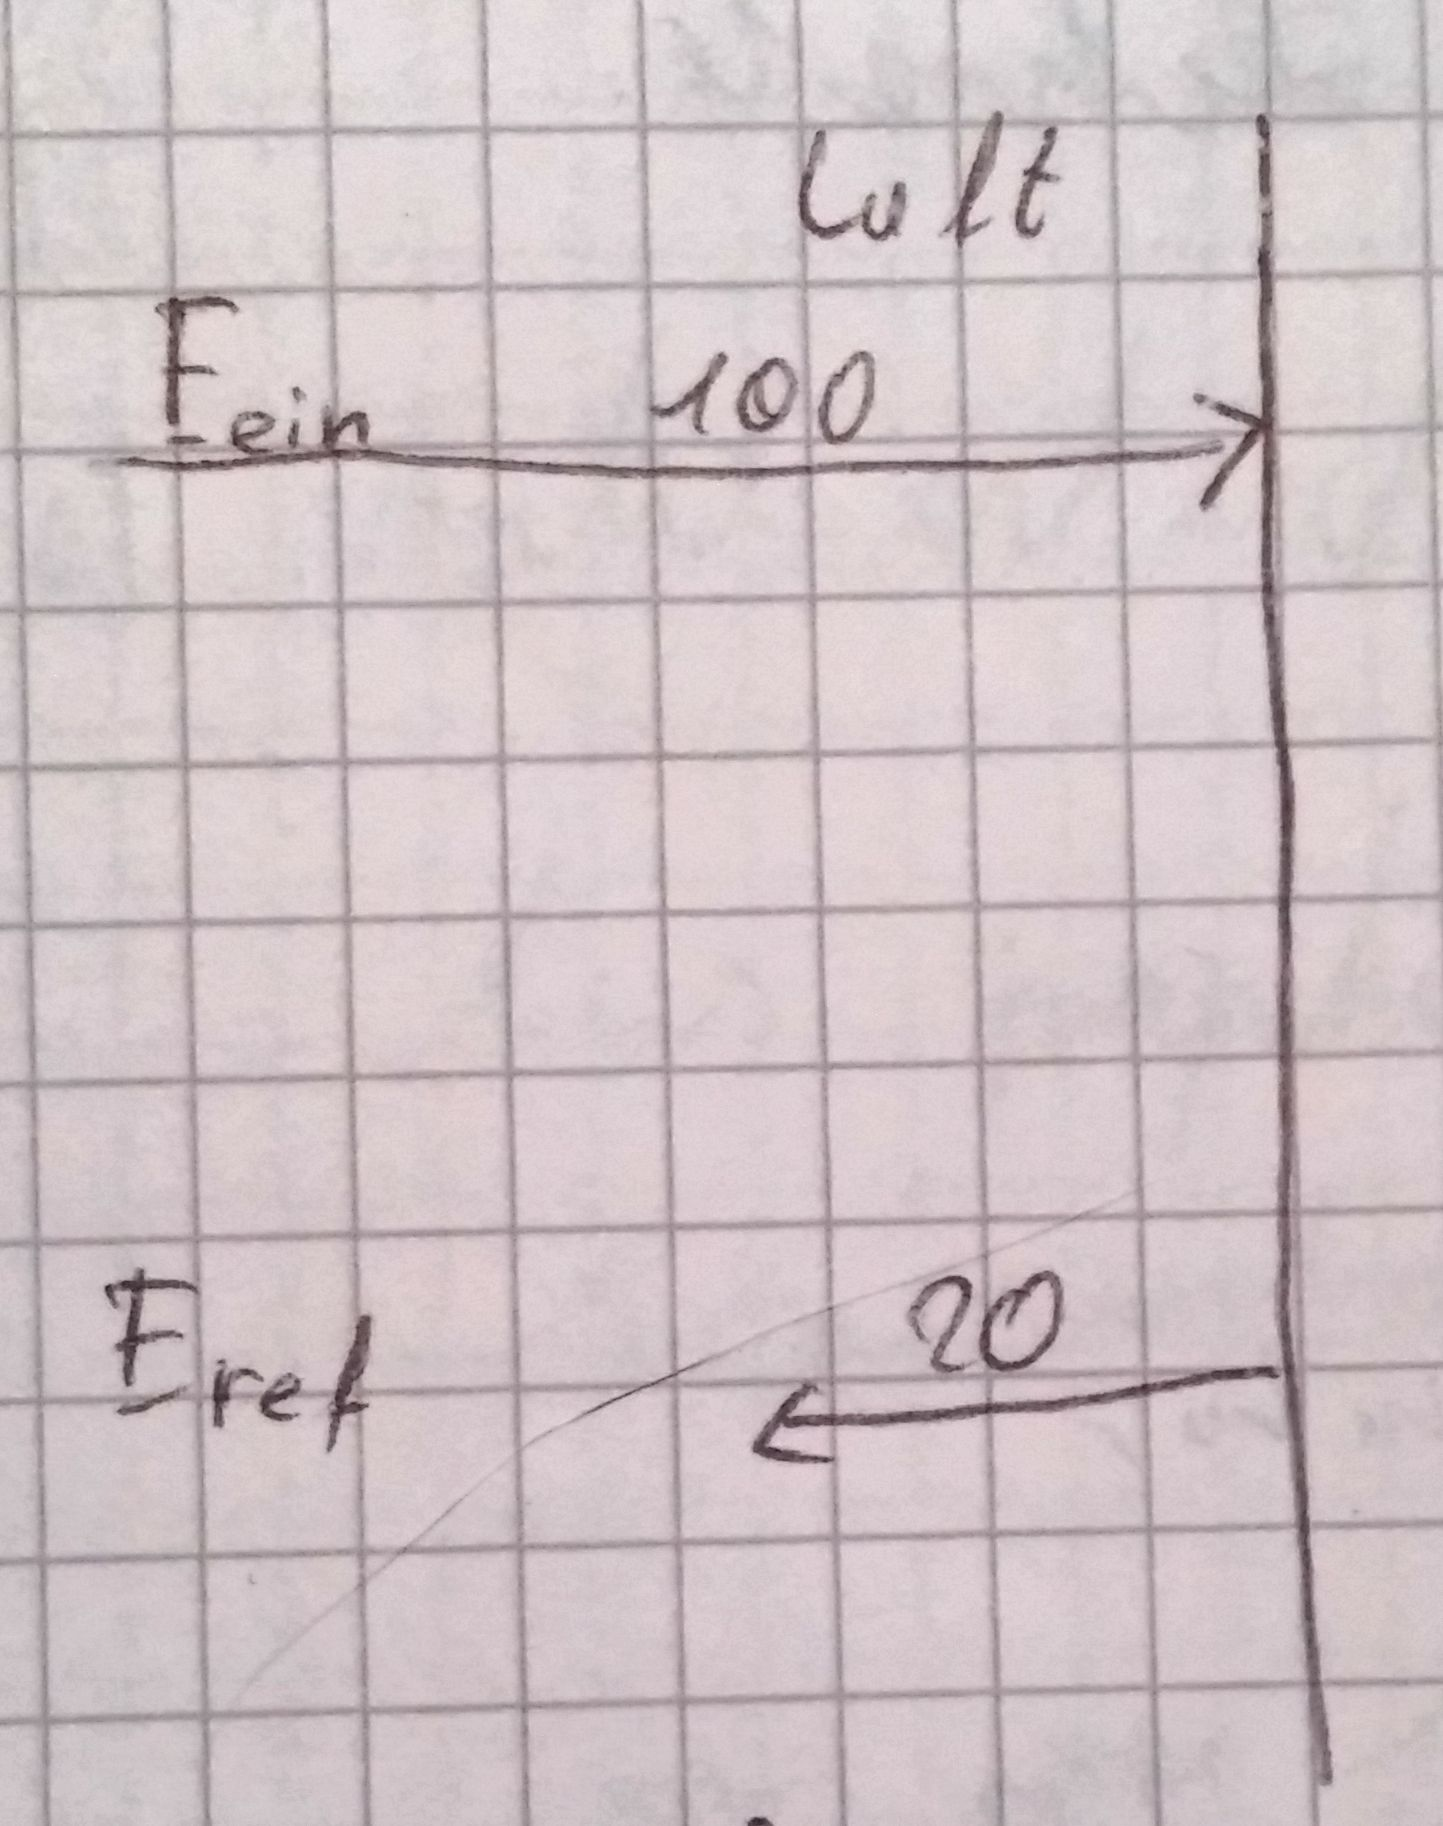
\includegraphics[width=5cm]{A1_1.jpg}
	\end{minipage}
	\hfill
	\begin{minipage}[hbt]{7cm}
		\centering
		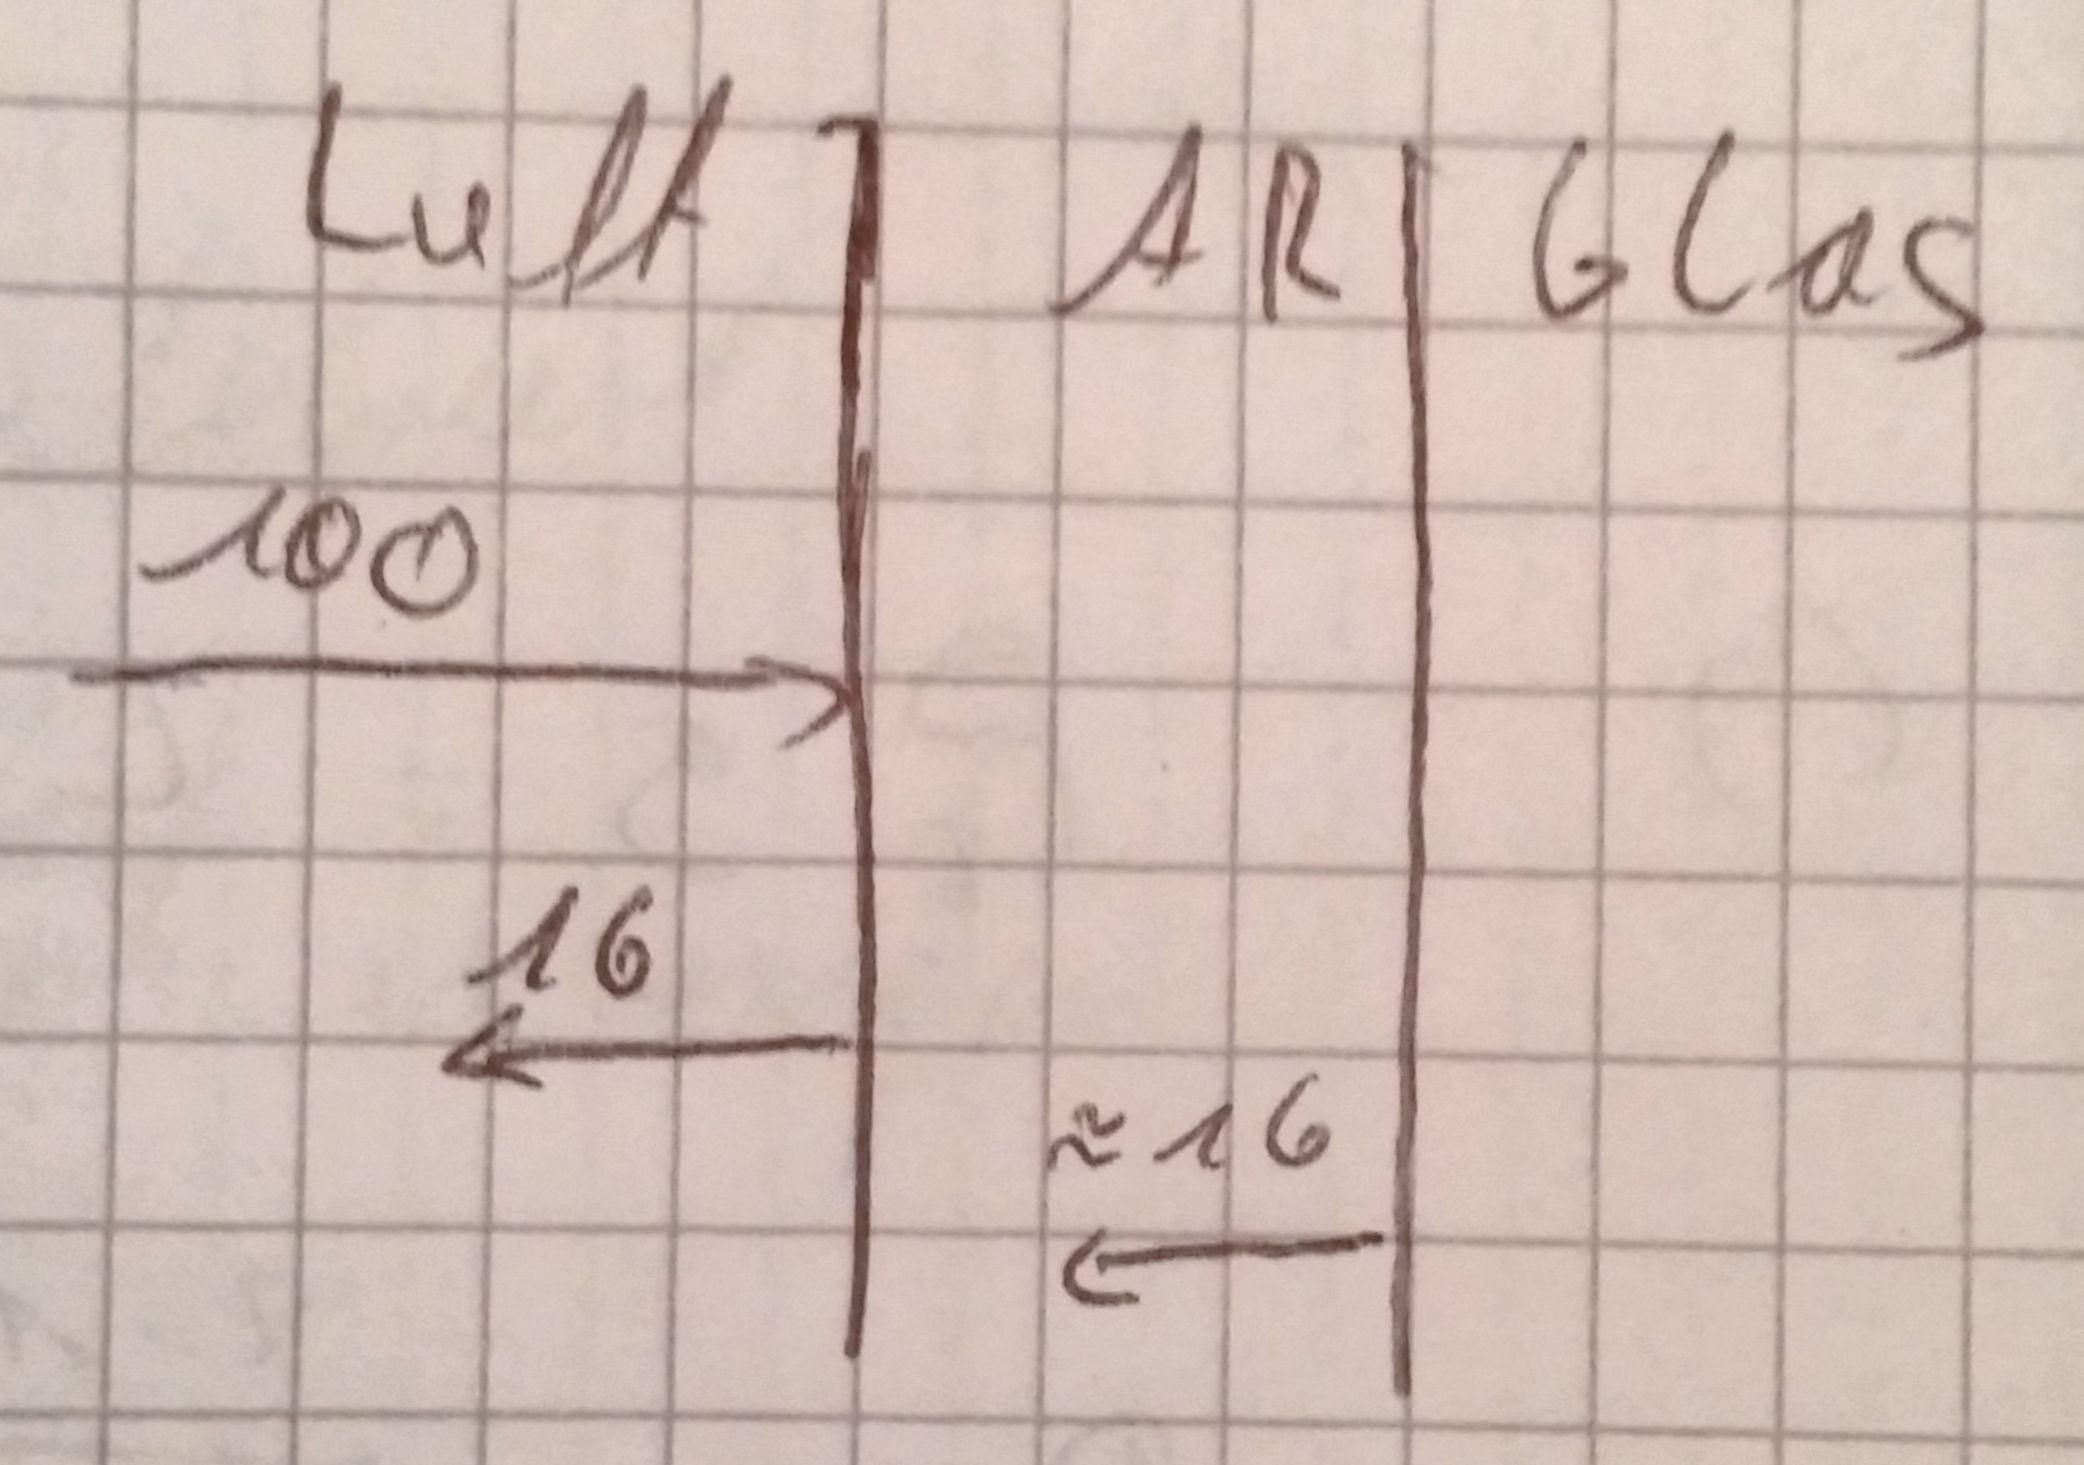
\includegraphics[width=7cm]{A1_2.jpg}
	\end{minipage}
\end{figure}


Bei dem Glas ohne Reflexionsschicht erhalten wir nach $I \sim E^2$:

\begin{align*}
0,2^2 = 0,04 = \unit[4]{\%}
\intertext{Bei Glas mit Reflexionsschicht gilt für den Reflexionsgrad:}
R &= \frac{1,38 - 1}{1,38 + 1} = 0,159 = \unit[16]{\%} = E_0
\intertext{Die intensität ist dann:}
A_{eff} &= 2 \cdot E_0 \cdot \cos \left( \frac{\phi}{2} \right) = 32 \cdot \cos \left( \frac{\phi}{2} \right) \\
I &\sim A_{eff}^2 = 4 \cdot E_0^2 \cdot \cos^2 \left( \frac{\phi}{2} \right)
\end{align*}

Wenn wir uns die Phasenverschiebung mit $\frac{\pi \cdot 550}{\lambda}$ anschauen, dann erkennen wir, dass sich die Phasenverschiebung zu kleinen Wellenlängen stärker ändert als zu großen.










\end{document}